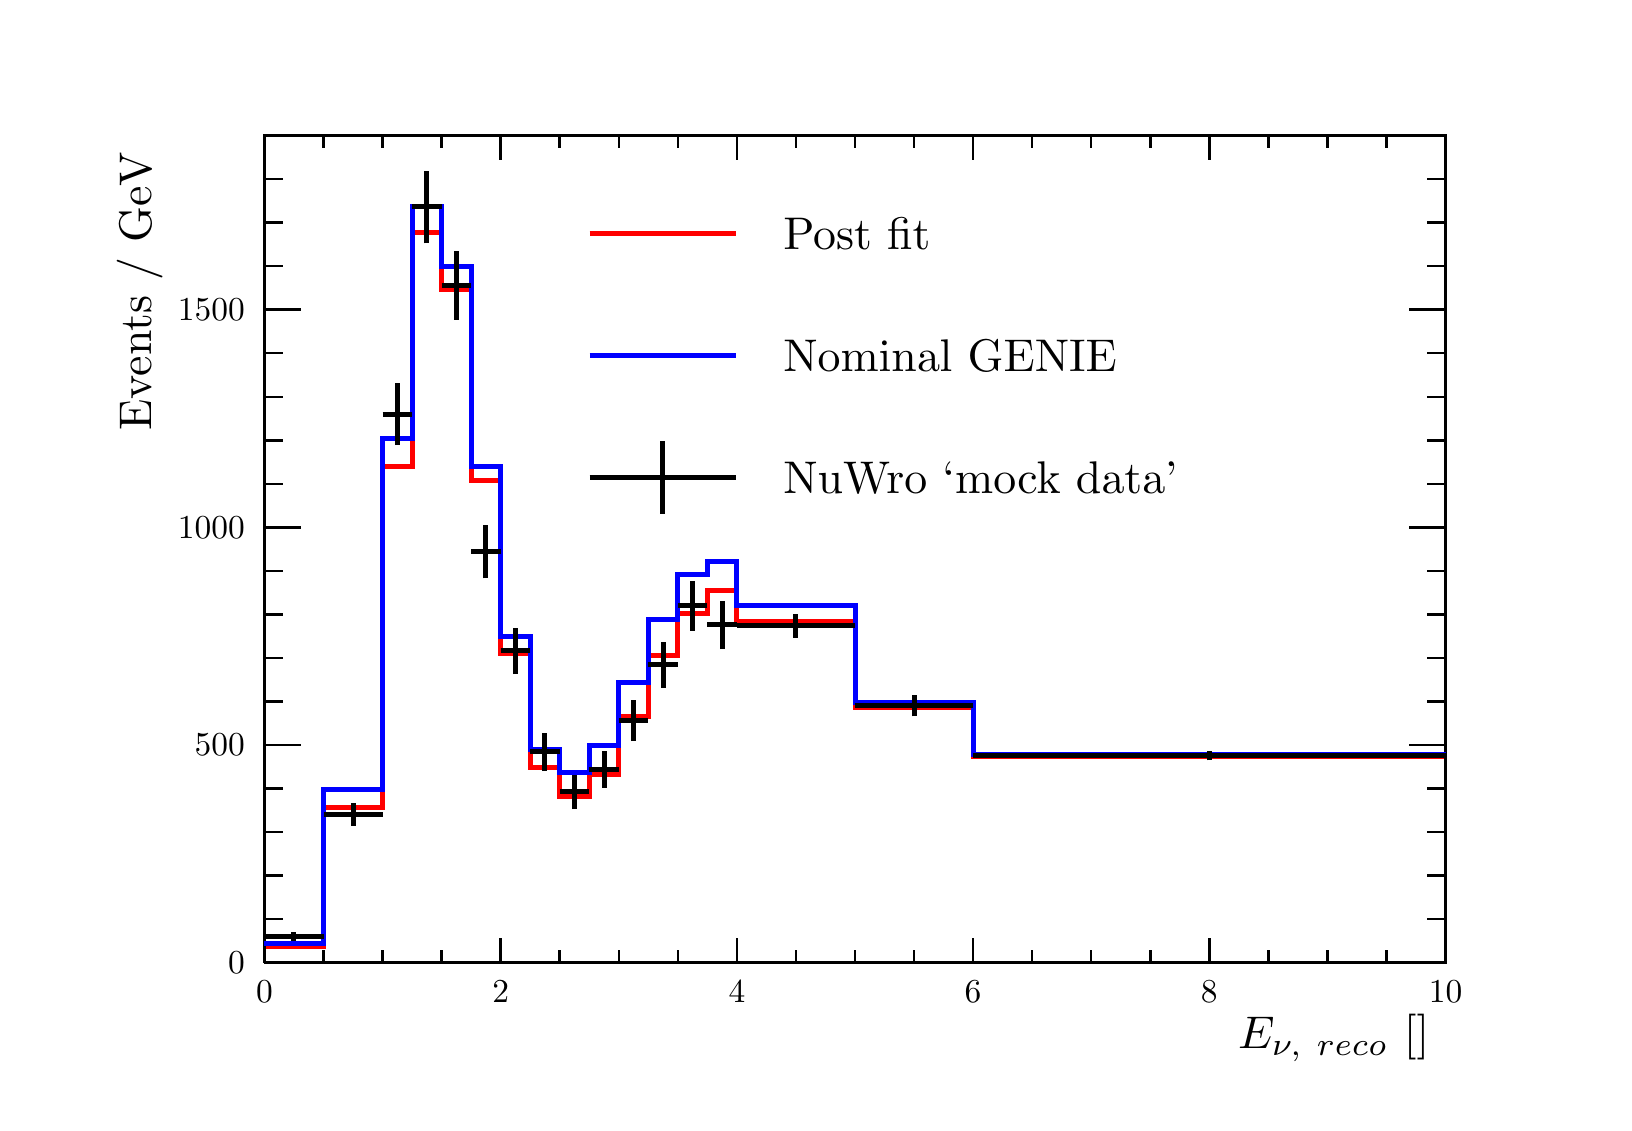
\begin{tikzpicture}
\pgfdeclareplotmark{cross} {
\pgfpathmoveto{\pgfpoint{-0.3\pgfplotmarksize}{\pgfplotmarksize}}
\pgfpathlineto{\pgfpoint{+0.3\pgfplotmarksize}{\pgfplotmarksize}}
\pgfpathlineto{\pgfpoint{+0.3\pgfplotmarksize}{0.3\pgfplotmarksize}}
\pgfpathlineto{\pgfpoint{+1\pgfplotmarksize}{0.3\pgfplotmarksize}}
\pgfpathlineto{\pgfpoint{+1\pgfplotmarksize}{-0.3\pgfplotmarksize}}
\pgfpathlineto{\pgfpoint{+0.3\pgfplotmarksize}{-0.3\pgfplotmarksize}}
\pgfpathlineto{\pgfpoint{+0.3\pgfplotmarksize}{-1.\pgfplotmarksize}}
\pgfpathlineto{\pgfpoint{-0.3\pgfplotmarksize}{-1.\pgfplotmarksize}}
\pgfpathlineto{\pgfpoint{-0.3\pgfplotmarksize}{-0.3\pgfplotmarksize}}
\pgfpathlineto{\pgfpoint{-1.\pgfplotmarksize}{-0.3\pgfplotmarksize}}
\pgfpathlineto{\pgfpoint{-1.\pgfplotmarksize}{0.3\pgfplotmarksize}}
\pgfpathlineto{\pgfpoint{-0.3\pgfplotmarksize}{0.3\pgfplotmarksize}}
\pgfpathclose
\pgfusepathqstroke
}
\pgfdeclareplotmark{cross*} {
\pgfpathmoveto{\pgfpoint{-0.3\pgfplotmarksize}{\pgfplotmarksize}}
\pgfpathlineto{\pgfpoint{+0.3\pgfplotmarksize}{\pgfplotmarksize}}
\pgfpathlineto{\pgfpoint{+0.3\pgfplotmarksize}{0.3\pgfplotmarksize}}
\pgfpathlineto{\pgfpoint{+1\pgfplotmarksize}{0.3\pgfplotmarksize}}
\pgfpathlineto{\pgfpoint{+1\pgfplotmarksize}{-0.3\pgfplotmarksize}}
\pgfpathlineto{\pgfpoint{+0.3\pgfplotmarksize}{-0.3\pgfplotmarksize}}
\pgfpathlineto{\pgfpoint{+0.3\pgfplotmarksize}{-1.\pgfplotmarksize}}
\pgfpathlineto{\pgfpoint{-0.3\pgfplotmarksize}{-1.\pgfplotmarksize}}
\pgfpathlineto{\pgfpoint{-0.3\pgfplotmarksize}{-0.3\pgfplotmarksize}}
\pgfpathlineto{\pgfpoint{-1.\pgfplotmarksize}{-0.3\pgfplotmarksize}}
\pgfpathlineto{\pgfpoint{-1.\pgfplotmarksize}{0.3\pgfplotmarksize}}
\pgfpathlineto{\pgfpoint{-0.3\pgfplotmarksize}{0.3\pgfplotmarksize}}
\pgfpathclose
\pgfusepathqfillstroke
}
\pgfdeclareplotmark{newstar} {
\pgfpathmoveto{\pgfqpoint{0pt}{\pgfplotmarksize}}
\pgfpathlineto{\pgfqpointpolar{44}{0.5\pgfplotmarksize}}
\pgfpathlineto{\pgfqpointpolar{18}{\pgfplotmarksize}}
\pgfpathlineto{\pgfqpointpolar{-20}{0.5\pgfplotmarksize}}
\pgfpathlineto{\pgfqpointpolar{-54}{\pgfplotmarksize}}
\pgfpathlineto{\pgfqpointpolar{-90}{0.5\pgfplotmarksize}}
\pgfpathlineto{\pgfqpointpolar{234}{\pgfplotmarksize}}
\pgfpathlineto{\pgfqpointpolar{198}{0.5\pgfplotmarksize}}
\pgfpathlineto{\pgfqpointpolar{162}{\pgfplotmarksize}}
\pgfpathlineto{\pgfqpointpolar{134}{0.5\pgfplotmarksize}}
\pgfpathclose
\pgfusepathqstroke
}
\pgfdeclareplotmark{newstar*} {
\pgfpathmoveto{\pgfqpoint{0pt}{\pgfplotmarksize}}
\pgfpathlineto{\pgfqpointpolar{44}{0.5\pgfplotmarksize}}
\pgfpathlineto{\pgfqpointpolar{18}{\pgfplotmarksize}}
\pgfpathlineto{\pgfqpointpolar{-20}{0.5\pgfplotmarksize}}
\pgfpathlineto{\pgfqpointpolar{-54}{\pgfplotmarksize}}
\pgfpathlineto{\pgfqpointpolar{-90}{0.5\pgfplotmarksize}}
\pgfpathlineto{\pgfqpointpolar{234}{\pgfplotmarksize}}
\pgfpathlineto{\pgfqpointpolar{198}{0.5\pgfplotmarksize}}
\pgfpathlineto{\pgfqpointpolar{162}{\pgfplotmarksize}}
\pgfpathlineto{\pgfqpointpolar{134}{0.5\pgfplotmarksize}}
\pgfpathclose
\pgfusepathqfillstroke
}
\definecolor{c}{rgb}{1,1,1};
\draw [color=c, fill=c] (0,0) rectangle (20,13.639);
\draw [color=c, fill=c] (3,1.77307) rectangle (18,12.2751);
\definecolor{c}{rgb}{0,0,0};
\draw [c,line width=0.9] (3,1.77307) -- (3,12.2751) -- (18,12.2751) -- (18,1.77307) -- (3,1.77307);
\definecolor{c}{rgb}{1,1,1};
\draw [color=c, fill=c] (3,1.77307) rectangle (18,12.2751);
\definecolor{c}{rgb}{0,0,0};
\draw [c,line width=0.9] (3,1.77307) -- (3,12.2751) -- (18,12.2751) -- (18,1.77307) -- (3,1.77307);
\definecolor{c}{rgb}{1,0,0};
\draw [c,line width=1.8] (3,1.97612) -- (3.75,1.97612) -- (3.75,3.7388) -- (4.5,3.7388) -- (4.5,8.06904) -- (4.875,8.06904) -- (4.875,11.0387) -- (5.25,11.0387) -- (5.25,10.3229) -- (5.625,10.3229) -- (5.625,7.89158) -- (6,7.89158) -- (6,5.69873) --
 (6.375,5.69873) -- (6.375,4.25038) -- (6.75,4.25038) -- (6.75,3.88247) -- (7.125,3.88247) -- (7.125,4.15842) -- (7.5,4.15842) -- (7.5,4.90241) -- (7.875,4.90241) -- (7.875,5.67058) -- (8.25,5.67058) -- (8.25,6.20216) -- (8.625,6.20216) --
 (8.625,6.49336) -- (9,6.49336) -- (9,6.10497) -- (10.5,6.10497) -- (10.5,5.01554) -- (12,5.01554) -- (12,4.39275) -- (18,4.39275);
\definecolor{c}{rgb}{0,0,0};
\draw [c,line width=0.9] (3,1.77307) -- (18,1.77307);
\draw [c,line width=0.9] (3,2.07994) -- (3,1.77307);
\draw [c,line width=0.9] (3.75,1.9265) -- (3.75,1.77307);
\draw [c,line width=0.9] (4.5,1.9265) -- (4.5,1.77307);
\draw [c,line width=0.9] (5.25,1.9265) -- (5.25,1.77307);
\draw [c,line width=0.9] (6,2.07994) -- (6,1.77307);
\draw [c,line width=0.9] (6.75,1.9265) -- (6.75,1.77307);
\draw [c,line width=0.9] (7.5,1.9265) -- (7.5,1.77307);
\draw [c,line width=0.9] (8.25,1.9265) -- (8.25,1.77307);
\draw [c,line width=0.9] (9,2.07994) -- (9,1.77307);
\draw [c,line width=0.9] (9.75,1.9265) -- (9.75,1.77307);
\draw [c,line width=0.9] (10.5,1.9265) -- (10.5,1.77307);
\draw [c,line width=0.9] (11.25,1.9265) -- (11.25,1.77307);
\draw [c,line width=0.9] (12,2.07994) -- (12,1.77307);
\draw [c,line width=0.9] (12.75,1.9265) -- (12.75,1.77307);
\draw [c,line width=0.9] (13.5,1.9265) -- (13.5,1.77307);
\draw [c,line width=0.9] (14.25,1.9265) -- (14.25,1.77307);
\draw [c,line width=0.9] (15,2.07994) -- (15,1.77307);
\draw [c,line width=0.9] (15.75,1.9265) -- (15.75,1.77307);
\draw [c,line width=0.9] (16.5,1.9265) -- (16.5,1.77307);
\draw [c,line width=0.9] (17.25,1.9265) -- (17.25,1.77307);
\draw [c,line width=0.9] (18,2.07994) -- (18,1.77307);
\draw [anchor=base] (3,1.26842) node[scale=1.20912, color=c, rotate=0]{0};
\draw [anchor=base] (6,1.26842) node[scale=1.20912, color=c, rotate=0]{2};
\draw [anchor=base] (9,1.26842) node[scale=1.20912, color=c, rotate=0]{4};
\draw [anchor=base] (12,1.26842) node[scale=1.20912, color=c, rotate=0]{6};
\draw [anchor=base] (15,1.26842) node[scale=1.20912, color=c, rotate=0]{8};
\draw [anchor=base] (18,1.26842) node[scale=1.20912, color=c, rotate=0]{10};
\draw [anchor= east] (18,0.812882) node[scale=1.65459, color=c, rotate=0]{$E_{\nu,~\text{reco}}$ [\si{\GeV}]};
\draw [c,line width=0.9] (3,12.2751) -- (18,12.2751);
\draw [c,line width=0.9] (3,11.9682) -- (3,12.2751);
\draw [c,line width=0.9] (3.75,12.1216) -- (3.75,12.2751);
\draw [c,line width=0.9] (4.5,12.1216) -- (4.5,12.2751);
\draw [c,line width=0.9] (5.25,12.1216) -- (5.25,12.2751);
\draw [c,line width=0.9] (6,11.9682) -- (6,12.2751);
\draw [c,line width=0.9] (6.75,12.1216) -- (6.75,12.2751);
\draw [c,line width=0.9] (7.5,12.1216) -- (7.5,12.2751);
\draw [c,line width=0.9] (8.25,12.1216) -- (8.25,12.2751);
\draw [c,line width=0.9] (9,11.9682) -- (9,12.2751);
\draw [c,line width=0.9] (9.75,12.1216) -- (9.75,12.2751);
\draw [c,line width=0.9] (10.5,12.1216) -- (10.5,12.2751);
\draw [c,line width=0.9] (11.25,12.1216) -- (11.25,12.2751);
\draw [c,line width=0.9] (12,11.9682) -- (12,12.2751);
\draw [c,line width=0.9] (12.75,12.1216) -- (12.75,12.2751);
\draw [c,line width=0.9] (13.5,12.1216) -- (13.5,12.2751);
\draw [c,line width=0.9] (14.25,12.1216) -- (14.25,12.2751);
\draw [c,line width=0.9] (15,11.9682) -- (15,12.2751);
\draw [c,line width=0.9] (15.75,12.1216) -- (15.75,12.2751);
\draw [c,line width=0.9] (16.5,12.1216) -- (16.5,12.2751);
\draw [c,line width=0.9] (17.25,12.1216) -- (17.25,12.2751);
\draw [c,line width=0.9] (18,11.9682) -- (18,12.2751);
\draw [c,line width=0.9] (3,1.77307) -- (3,12.2751);
\draw [c,line width=0.9] (3.462,1.77307) -- (3,1.77307);
\draw [c,line width=0.9] (3.231,2.3258) -- (3,2.3258);
\draw [c,line width=0.9] (3.231,2.87854) -- (3,2.87854);
\draw [c,line width=0.9] (3.231,3.43128) -- (3,3.43128);
\draw [c,line width=0.9] (3.231,3.98401) -- (3,3.98401);
\draw [c,line width=0.9] (3.462,4.53675) -- (3,4.53675);
\draw [c,line width=0.9] (3.231,5.08949) -- (3,5.08949);
\draw [c,line width=0.9] (3.231,5.64223) -- (3,5.64223);
\draw [c,line width=0.9] (3.231,6.19496) -- (3,6.19496);
\draw [c,line width=0.9] (3.231,6.7477) -- (3,6.7477);
\draw [c,line width=0.9] (3.462,7.30044) -- (3,7.30044);
\draw [c,line width=0.9] (3.231,7.85317) -- (3,7.85317);
\draw [c,line width=0.9] (3.231,8.40591) -- (3,8.40591);
\draw [c,line width=0.9] (3.231,8.95865) -- (3,8.95865);
\draw [c,line width=0.9] (3.231,9.51139) -- (3,9.51139);
\draw [c,line width=0.9] (3.462,10.0641) -- (3,10.0641);
\draw [c,line width=0.9] (3.462,10.0641) -- (3,10.0641);
\draw [c,line width=0.9] (3.231,10.6169) -- (3,10.6169);
\draw [c,line width=0.9] (3.231,11.1696) -- (3,11.1696);
\draw [c,line width=0.9] (3.231,11.7223) -- (3,11.7223);
\draw [c,line width=0.9] (3.231,12.2751) -- (3,12.2751);
\draw [anchor= east] (2.9,1.77307) node[scale=1.20912, color=c, rotate=0]{0};
\draw [anchor= east] (2.9,4.53675) node[scale=1.20912, color=c, rotate=0]{500};
\draw [anchor= east] (2.9,7.30044) node[scale=1.20912, color=c, rotate=0]{1000};
\draw [anchor= east] (2.9,10.0641) node[scale=1.20912, color=c, rotate=0]{1500};
\draw [anchor= east] (1.416,12.2751) node[scale=1.65459, color=c, rotate=90]{Events / GeV};
\draw [c,line width=0.9] (18,1.77307) -- (18,12.2751);
\draw [c,line width=0.9] (17.538,1.77307) -- (18,1.77307);
\draw [c,line width=0.9] (17.769,2.3258) -- (18,2.3258);
\draw [c,line width=0.9] (17.769,2.87854) -- (18,2.87854);
\draw [c,line width=0.9] (17.769,3.43128) -- (18,3.43128);
\draw [c,line width=0.9] (17.769,3.98401) -- (18,3.98401);
\draw [c,line width=0.9] (17.538,4.53675) -- (18,4.53675);
\draw [c,line width=0.9] (17.769,5.08949) -- (18,5.08949);
\draw [c,line width=0.9] (17.769,5.64223) -- (18,5.64223);
\draw [c,line width=0.9] (17.769,6.19496) -- (18,6.19496);
\draw [c,line width=0.9] (17.769,6.7477) -- (18,6.7477);
\draw [c,line width=0.9] (17.538,7.30044) -- (18,7.30044);
\draw [c,line width=0.9] (17.769,7.85317) -- (18,7.85317);
\draw [c,line width=0.9] (17.769,8.40591) -- (18,8.40591);
\draw [c,line width=0.9] (17.769,8.95865) -- (18,8.95865);
\draw [c,line width=0.9] (17.769,9.51139) -- (18,9.51139);
\draw [c,line width=0.9] (17.538,10.0641) -- (18,10.0641);
\draw [c,line width=0.9] (17.538,10.0641) -- (18,10.0641);
\draw [c,line width=0.9] (17.769,10.6169) -- (18,10.6169);
\draw [c,line width=0.9] (17.769,11.1696) -- (18,11.1696);
\draw [c,line width=0.9] (17.769,11.7223) -- (18,11.7223);
\draw [c,line width=0.9] (17.769,12.2751) -- (18,12.2751);
\definecolor{c}{rgb}{0,0,1};
\draw [c,line width=1.8] (3,2.01055) -- (3.75,2.01055) -- (3.75,3.96457) -- (4.5,3.96457) -- (4.5,8.43143) -- (4.875,8.43143) -- (4.875,11.3693) -- (5.25,11.3693) -- (5.25,10.609) -- (5.625,10.609) -- (5.625,8.0773) -- (6,8.0773) -- (6,5.91515) --
 (6.375,5.91515) -- (6.375,4.48277) -- (6.75,4.48277) -- (6.75,4.18381) -- (7.125,4.18381) -- (7.125,4.53513) -- (7.5,4.53513) -- (7.5,5.33483) -- (7.875,5.33483) -- (7.875,6.13383) -- (8.25,6.13383) -- (8.25,6.70392) -- (8.625,6.70392) --
 (8.625,6.86182) -- (9,6.86182) -- (9,6.31204) -- (10.5,6.31204) -- (10.5,5.07409) -- (12,5.07409) -- (12,4.41756) -- (18,4.41756);
\definecolor{c}{rgb}{0,0,0};
\draw [c,line width=1.8] (3.375,2.04416) -- (3.375,2.10471);
\draw [c,line width=1.8] (3.375,2.10471) -- (3.375,2.16526);
\draw [c,line width=1.8] (3,2.10471) -- (3.375,2.10471);
\draw [c,line width=1.8] (3.375,2.10471) -- (3.75,2.10471);
\foreach \P in {(3.375,2.10471)}{\draw[mark options={color=c,fill=c},mark size=2.402402pt, line width=0.000000pt, mark=*,mark size=1pt] plot coordinates {\P};}
\draw [c,line width=1.8] (4.125,3.50824) -- (4.125,3.65237);
\draw [c,line width=1.8] (4.125,3.65237) -- (4.125,3.79651);
\draw [c,line width=1.8] (3.75,3.65237) -- (4.125,3.65237);
\draw [c,line width=1.8] (4.125,3.65237) -- (4.5,3.65237);
\foreach \P in {(4.125,3.65237)}{\draw[mark options={color=c,fill=c},mark size=2.402402pt, line width=0.000000pt, mark=*,mark size=1pt] plot coordinates {\P};}
\draw [c,line width=1.8] (4.6875,8.34515) -- (4.6875,8.73755);
\draw [c,line width=1.8] (4.6875,8.73755) -- (4.6875,9.12996);
\draw [c,line width=1.8] (4.5,8.73755) -- (4.6875,8.73755);
\draw [c,line width=1.8] (4.6875,8.73755) -- (4.875,8.73755);
\foreach \P in {(4.6875,8.73755)}{\draw[mark options={color=c,fill=c},mark size=2.402402pt, line width=0.000000pt, mark=*,mark size=1pt] plot coordinates {\P};}
\draw [c,line width=1.8] (5.0625,10.908) -- (5.0625,11.3686);
\draw [c,line width=1.8] (5.0625,11.3686) -- (5.0625,11.8292);
\draw [c,line width=1.8] (4.875,11.3686) -- (5.0625,11.3686);
\draw [c,line width=1.8] (5.0625,11.3686) -- (5.25,11.3686);
\foreach \P in {(5.0625,11.3686)}{\draw[mark options={color=c,fill=c},mark size=2.402402pt, line width=0.000000pt, mark=*,mark size=1pt] plot coordinates {\P};}
\draw [c,line width=1.8] (5.4375,9.93759) -- (5.4375,10.3737);
\draw [c,line width=1.8] (5.4375,10.3737) -- (5.4375,10.8097);
\draw [c,line width=1.8] (5.25,10.3737) -- (5.4375,10.3737);
\draw [c,line width=1.8] (5.4375,10.3737) -- (5.625,10.3737);
\foreach \P in {(5.4375,10.3737)}{\draw[mark options={color=c,fill=c},mark size=2.402402pt, line width=0.000000pt, mark=*,mark size=1pt] plot coordinates {\P};}
\draw [c,line width=1.8] (5.8125,6.65125) -- (5.8125,6.9909);
\draw [c,line width=1.8] (5.8125,6.9909) -- (5.8125,7.33056);
\draw [c,line width=1.8] (5.625,6.9909) -- (5.8125,6.9909);
\draw [c,line width=1.8] (5.8125,6.9909) -- (6,6.9909);
\foreach \P in {(5.8125,6.9909)}{\draw[mark options={color=c,fill=c},mark size=2.402402pt, line width=0.000000pt, mark=*,mark size=1pt] plot coordinates {\P};}
\draw [c,line width=1.8] (6.1875,5.43486) -- (6.1875,5.73066);
\draw [c,line width=1.8] (6.1875,5.73066) -- (6.1875,6.02647);
\draw [c,line width=1.8] (6,5.73066) -- (6.1875,5.73066);
\draw [c,line width=1.8] (6.1875,5.73066) -- (6.375,5.73066);
\foreach \P in {(6.1875,5.73066)}{\draw[mark options={color=c,fill=c},mark size=2.402402pt, line width=0.000000pt, mark=*,mark size=1pt] plot coordinates {\P};}
\draw [c,line width=1.8] (6.5625,4.20511) -- (6.5625,4.44831);
\draw [c,line width=1.8] (6.5625,4.44831) -- (6.5625,4.69152);
\draw [c,line width=1.8] (6.375,4.44831) -- (6.5625,4.44831);
\draw [c,line width=1.8] (6.5625,4.44831) -- (6.75,4.44831);
\foreach \P in {(6.5625,4.44831)}{\draw[mark options={color=c,fill=c},mark size=2.402402pt, line width=0.000000pt, mark=*,mark size=1pt] plot coordinates {\P};}
\draw [c,line width=1.8] (6.9375,3.72092) -- (6.9375,3.9398);
\draw [c,line width=1.8] (6.9375,3.9398) -- (6.9375,4.15867);
\draw [c,line width=1.8] (6.75,3.9398) -- (6.9375,3.9398);
\draw [c,line width=1.8] (6.9375,3.9398) -- (7.125,3.9398);
\foreach \P in {(6.9375,3.9398)}{\draw[mark options={color=c,fill=c},mark size=2.402402pt, line width=0.000000pt, mark=*,mark size=1pt] plot coordinates {\P};}
\draw [c,line width=1.8] (7.3125,3.99428) -- (7.3125,4.22722);
\draw [c,line width=1.8] (7.3125,4.22722) -- (7.3125,4.46016);
\draw [c,line width=1.8] (7.125,4.22722) -- (7.3125,4.22722);
\draw [c,line width=1.8] (7.3125,4.22722) -- (7.5,4.22722);
\foreach \P in {(7.3125,4.22722)}{\draw[mark options={color=c,fill=c},mark size=2.402402pt, line width=0.000000pt, mark=*,mark size=1pt] plot coordinates {\P};}
\draw [c,line width=1.8] (7.6875,4.58562) -- (7.6875,4.84628);
\draw [c,line width=1.8] (7.6875,4.84628) -- (7.6875,5.10695);
\draw [c,line width=1.8] (7.5,4.84628) -- (7.6875,4.84628);
\draw [c,line width=1.8] (7.6875,4.84628) -- (7.875,4.84628);
\foreach \P in {(7.6875,4.84628)}{\draw[mark options={color=c,fill=c},mark size=2.402402pt, line width=0.000000pt, mark=*,mark size=1pt] plot coordinates {\P};}
\draw [c,line width=1.8] (8.0625,5.26467) -- (8.0625,5.55379);
\draw [c,line width=1.8] (8.0625,5.55379) -- (8.0625,5.84291);
\draw [c,line width=1.8] (7.875,5.55379) -- (8.0625,5.55379);
\draw [c,line width=1.8] (8.0625,5.55379) -- (8.25,5.55379);
\foreach \P in {(8.0625,5.55379)}{\draw[mark options={color=c,fill=c},mark size=2.402402pt, line width=0.000000pt, mark=*,mark size=1pt] plot coordinates {\P};}
\draw [c,line width=1.8] (8.4375,5.98895) -- (8.4375,6.30551);
\draw [c,line width=1.8] (8.4375,6.30551) -- (8.4375,6.62207);
\draw [c,line width=1.8] (8.25,6.30551) -- (8.4375,6.30551);
\draw [c,line width=1.8] (8.4375,6.30551) -- (8.625,6.30551);
\foreach \P in {(8.4375,6.30551)}{\draw[mark options={color=c,fill=c},mark size=2.402402pt, line width=0.000000pt, mark=*,mark size=1pt] plot coordinates {\P};}
\draw [c,line width=1.8] (8.8125,5.75436) -- (8.8125,6.06231);
\draw [c,line width=1.8] (8.8125,6.06231) -- (8.8125,6.37026);
\draw [c,line width=1.8] (8.625,6.06231) -- (8.8125,6.06231);
\draw [c,line width=1.8] (8.8125,6.06231) -- (9,6.06231);
\foreach \P in {(8.8125,6.06231)}{\draw[mark options={color=c,fill=c},mark size=2.402402pt, line width=0.000000pt, mark=*,mark size=1pt] plot coordinates {\P};}
\draw [c,line width=1.8] (9.75,5.89748) -- (9.75,6.05125);
\draw [c,line width=1.8] (9.75,6.05125) -- (9.75,6.20503);
\draw [c,line width=1.8] (9,6.05125) -- (9.75,6.05125);
\draw [c,line width=1.8] (9.75,6.05125) -- (10.5,6.05125);
\foreach \P in {(9.75,6.05125)}{\draw[mark options={color=c,fill=c},mark size=2.402402pt, line width=0.000000pt, mark=*,mark size=1pt] plot coordinates {\P};}
\draw [c,line width=1.8] (11.25,4.89996) -- (11.25,5.03421);
\draw [c,line width=1.8] (11.25,5.03421) -- (11.25,5.16847);
\draw [c,line width=1.8] (10.5,5.03421) -- (11.25,5.03421);
\draw [c,line width=1.8] (11.25,5.03421) -- (12,5.03421);
\foreach \P in {(11.25,5.03421)}{\draw[mark options={color=c,fill=c},mark size=2.402402pt, line width=0.000000pt, mark=*,mark size=1pt] plot coordinates {\P};}
\draw [c,line width=1.8] (15,4.34107) -- (15,4.40133);
\draw [c,line width=1.8] (15,4.40133) -- (15,4.4616);
\draw [c,line width=1.8] (12,4.40133) -- (15,4.40133);
\draw [c,line width=1.8] (15,4.40133) -- (18,4.40133);
\foreach \P in {(15,4.40133)}{\draw[mark options={color=c,fill=c},mark size=2.402402pt, line width=0.000000pt, mark=*,mark size=1pt] plot coordinates {\P};}
\definecolor{c}{rgb}{1,1,1};
\draw [color=c, fill=c] (2,12.8206) rectangle (18,13.5708);
\definecolor{c}{rgb}{0,0,0};
%\draw (10,13.1957) node[scale=1.40004, color=c, rotate=0]{$\nu_{\mu} RHC postfit: \delta = 1.57, \chi^{2} = 51.36$};
\definecolor{c}{rgb}{1,1,1};
\draw [color=c, fill=c] (6.73352,7.16332) rectangle (17.3352,11.8052);
\definecolor{c}{rgb}{0,0,0};
\draw [anchor= west] (9.38395,11.0315) node[scale=1.65459, color=c, rotate=0]{Post fit};
\definecolor{c}{rgb}{1,0,0};
\draw [c,line width=1.8] (7.13109,11.0315) -- (8.98639,11.0315);
\definecolor{c}{rgb}{0,0,0};
\draw [anchor= west] (9.38395,9.48424) node[scale=1.65459, color=c, rotate=0]{Nominal GENIE};
\definecolor{c}{rgb}{0,0,1};
\draw [c,line width=1.8] (7.13109,9.48424) -- (8.98639,9.48424);
\definecolor{c}{rgb}{0,0,0};
\draw [anchor= west] (9.38395,7.93696) node[scale=1.65459, color=c, rotate=0]{NuWro `mock data'};
\draw [c,line width=1.8] (7.13109,7.93696) -- (8.98639,7.93696);
\draw [c,line width=1.8] (8.05874,7.47278) -- (8.05874,8.40115);
\end{tikzpicture}
